\documentclass{article}

% if you need to pass options to natbib, use, e.g.:
%     \PassOptionsToPackage{numbers, compress}{natbib}
% before loading neurips_2021

% ready for submission
\PassOptionsToPackage{numbers, compress}{natbib}
\usepackage[final]{neurips_2021}

% to compile a preprint version, e.g., for submission to arXiv, add add the
% [preprint] option:
%     \usepackage[preprint]{neurips_2021}

% to compile a camera-ready version, add the [final] option, e.g.:
%\usepackage[final]{neurips_2021}

% to avoid loading the natbib package, add option nonatbib:
%    \usepackage[nonatbib]{neurips_2021}

\usepackage[utf8]{inputenc} % allow utf-8 input
\usepackage[T1]{fontenc}    % use 8-bit T1 fonts
\usepackage{hyperref}       % hyperlinks
\usepackage{url}            % simple URL typesetting
\usepackage{booktabs}       % professional-quality tables
\usepackage{amsfonts}       % blackboard math symbols
\usepackage{nicefrac}       % compact symbols for 1/2, etc.
\usepackage{microtype}      % microtypography
\usepackage{xcolor}         % colors
\usepackage{tikz}
\usepackage{amsmath}
\usepackage{mathtools}
\usepackage{bbm}
\usepackage{amssymb}


%bibliography
\bibliographystyle{plainnat}


\title{Automatic feature classification in stochastic block models}
% The \author macro works with any number of authors. There are two commands
% used to separate the names and addresses of multiple authors: \And and \AND.
%
% Using \And between authors leaves it to LaTeX to determine where to break the
% lines. Using \AND forces a line break at that point. So, if LaTeX puts 3 of 4
% authors names on the first line, and the last on the second line, try using
% \AND instead of \And before the third author name.

\author{
  Lawrence Tray \\
  Department of Engineering \\
  University of Cambridge \\
  \texttt{lpt30@cam.ac.uk} \\
  % examples of more authors
  \And
  Ioannis Kontoyiannis \\
  Department of Mathematics \\
  University of Cambridge \\
  \texttt{ik355@cam.ac.uk}
}

%custom commands
\newcommand{\Xcal}{\mathcal{X}}
\newcommand{\Bcal}{\mathcal{B}}
\newcommand{\Integers}{\mathbb{Z}}
\newcommand{\one}{\mathbbm{1}}
\newcommand{\Gaussian}{\mathcal{N}}
\newcommand{\indep}{\perp \!\!\! \perp}
\newcommand{\specialchoose}{\genfrac{\{}{\}}{0pt}{}}
\newcommand{\Expect}{\mathbb{E}}


%envs
\newtheorem{definition}{Definition}[section]
\newtheorem{theorem}{Theorem}[section]
\newtheorem{corollary}{Corollary}[theorem]
\newtheorem{lemma}[theorem]{Lemma}


\begin{document}

\maketitle

\begin{abstract}
  Paper abstract.
\end{abstract}


\section{Introduction}


\section{Preliminaries}

We will be using the microcanonical stochastic block model, proposed by \cite{Peixoto-Bayesian-Microcanonical}. A paraphrased definition is given below.

\begin{definition}[Microcanonical SBM]
	\label{defn:microcan-sbm}
	Let $N \in \Integers^{+}$ denote the number of vertices in our graph. The block memberships are denoted by a vector $b$ of length $N$ where each entry $b_i \in \{1, 2 \dots B\}$ where $B$ is the number of nonempty blocks. Let $e$ be a $B \times B$ matrix of edge counts between blocks ($e_{rs}$ is number of edges from block $r$ onto block $s$ - or twice that number if $r=s$). We restrict our analysis to undirected graphs so $e$ is symmetric. For a non-degree-corrected stochastic block model (NDC-SBM), we say that the graph $A$ is generated as follows:
	%
	\begin{equation}
		A \sim \textrm{NDC-SBM}_{\textrm{MC}} (b, e)
	\end{equation}
	%
	Where edges are placed at random but respecting the constraints imposed by $e$ and $b$. The additional parameters $N$ and $B$ are omitted as they are inferred from the shape ofs of $b$ and $e$. If we interpret $A$ as an adjacency matrix, then this constraint can be written formally as: $e_{rs} = \sum_{i=1}^{N} \sum_{j=1}^{N} A_{ij} \one \{b_i = r\} \one \{b_j = s\}$. However, this formulation does not tolerate high degree variation within blocks as is typical of real-world data. We therefore introduce the degree-corrected SBM (DC-SBM) which has an additional parameter $k$ which is a vector of length $N$ encoding the degree sequence ($k_i$ is the degree of vertex $i$). Therefore, we write:
	%
	\begin{equation}
		A \sim \textrm{DC-SBM}_{\textrm{MC}} (b, e, k)
	\end{equation}
	%
	This imposes the additional constraint that $k_i = \sum_{j=1}^{N} A_{ij}$. In what follows, we will always assume the degree-corrected model unless otherwise specified.
	
\end{definition}


\section{Latent block generative model}

We restrict our analysis to labelled, undirected graphs with $N$ nodes. We define the vector $x_i \in \Xcal^D$ as the feature vector for the $i$'th vertex. Each vertex has $D$ total features and we assume all entries take values from the same set $\Xcal$. For the majority of datasets we analyse, we deal with binary feature flags so $\Xcal = \{0, 1\}$. The feature vectors $\{x_i\}_{i=1}^{N}$ are subsumed into the $N \times D$ matrix $X$.

The proposed generative model is given in figure \ref{fig:lbgm}. We start, with the feature matrix X and generate a vector of block memberships $b$. The parameters of this generator are encapsulated by $\theta$. Each feature vector $x_i$ is treated independently and used to generate the block membership $b_i$. We choose a single softmax layer to model $p(b_i | x_i, \theta)$. More complex models are possible but then deriving meaning from inferred parameter distributions is complicated. Summarising, we can write $p(b | X, \theta)$ as follows:
%
\begin{equation}
	p(b| X, \theta) = \prod_{i=1}^{N} p(b_i | x_i, \theta) = \prod_{i=1}^{N} \phi_{b_i} (x_i; \theta)
	= \prod_{i=1}^{N} \frac{\exp\left(w_{b_i}^T \tilde{x}_i\right)}{\sum_{k=1}^{B} \exp \left( w_k^T \tilde{x}_i\right)}
\end{equation}
%
Where $\tilde{x} \coloneqq \left[x_1, x_2, \dots x_D, 1\right]^T$ is an augmented version of $x$ that allows for a bias term. The parameters $\theta$ just contain the $B \times (D+1)$ matrix of weight values or alternatively, $\theta = \{w_k\}_{k=1}^{B}$.

\begin{figure}[!h]
	\centering
	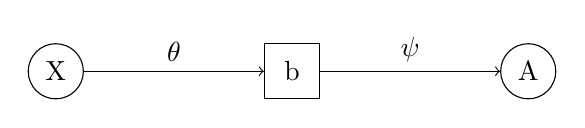
\begin{tikzpicture}[
		roundnode/.style={circle, draw=black, minimum size=7mm},
		squarednode/.style={rectangle, draw=black, minimum size=7mm}
		]
		% nodes
		\node[roundnode] (X) at (0, 0) {X};
		\node[squarednode] (b) at (3, 0) {b};
		\node[roundnode] (A) at (6, 0) {A};
		
		% arrows
		\draw[->] (X.east) -- node[above] {$\theta$} (b.west);
		\draw[->] (b.east) -- node[above] {$\psi$}(A.west);
	\end{tikzpicture}
	\caption{Latent block generative model}
	\label{fig:lbgm}
\end{figure}

Once we have generated the block memberships $b$, we proceed to draw the graph $A$ from the microcanical SBM (\ref{defn:microcan-sbm}) with additional parameters $\psi = \{e, k\}$. In a slight abuse of notation we denote the inter-block edge count matrix with $e = \psi_e$ and the degree sequence $k = \psi_k$ to make explicit that these are contained in $\psi$.
%
\begin{equation}
	A \sim \textrm{DC-SBM}_{\textrm{MC}} (b, \psi_e, \psi_k)
\end{equation}


\subsection{Prior selection}

Before performing any inference, we must specify priors on $\theta$ and $\psi$. For $\theta$ it seems sensible to choose a Gaussian prior, with zero mean and variance matrix $\sigma^2_\theta I$ such that each element of $\theta$ is independent and distributed like $\sim \Gaussian(0, \sigma)$. In vector form, the prior for $\theta$ is therefore:
%
\begin{equation}
	p(\theta) = \Gaussian \left( \theta ; 0, \sigma_\theta^2 I \right)
\end{equation}
%
We will see that this form of prior is equivalent to a regularisation term in neural network training that penalises extreme weight magnitudes. As $\sigma_\theta^2 \rightarrow \infty$ this becomes an uninformative uniform prior.

In our model $b$ is now an intermediate variable and so we cannot choose a prior. The closest thing we can get to a prior is $p(b | X)$. As far as inference on the right-hand-side of figure \ref{fig:lbgm}, we regard $p(b | X)$ as a pseudo-prior on $b$. We can show that our choice of prior for $p(\theta)$ leads to the following form for $p(b | X)$.
%
\begin{equation}
	p(b | X) = \int p(b | X, \theta) p(\theta) d\theta = B^{-N}
\end{equation}
%
In his paper, \citet{Peixoto-Bayesian-Microcanonical} proposes careful choices for the SBM parameters. The proposal is to write the joint prior on $(b, e, k)$ as a product of conditionals $p(b, e, k) = p(b) p(e | b) p(k | e, b)= p(b) p(\psi | b)$. For our purposes we must insert a conditioning on $X$, to form our pseudo-prior for $b$ and $\psi$.
%
\begin{equation}
	p(b, \psi | X) = p(b | X) p(\psi | b, X) = p(b | X) p(\psi | b)
\end{equation}
%
Where it is apparent by regarding figure \ref{fig:lbgm} as a Markov model that $(\psi \indep X) | b$. We then borrow the priors proposed by \citet{Peixoto-Bayesian-Microcanonical} for $p(\psi | b)$, repeated here for reference.
%
\begin{equation}
	p(\psi | b) = p(e | b) p(k | e, b) = \left[ \specialchoose{ \specialchoose{B}{2} }{ E} \right]^{-1} 
	\cdot \left[ \prod_r \frac{\prod_j \eta_j^r !}{n_r! q(e_r, n_r)} \right]
\end{equation}
%
Where $\specialchoose{n}{m}$ is shorthand for $\binom{n+m-1}{m} = \frac{(n+m-1)!}{(n-1)!(m)!}$ which can be thought of as the total number of histograms (non-negative bin values) with $n$ bins that are constrained to sum to $m$. $E = \frac{1}{2} \sum_{r,s} e_{rs}$ is the total number of edges. Importantly, $E$ is not allowed to vary and so $p(e|b)$ is uniform with respect to $e$. The variable $\eta_j^r$ is introduced to denote the number of vertices in block $r$ that have degree $j$. Formally, $\eta_j^r \coloneqq \sum_{i} \one\left\{b_i = r \right\} \one \left\{k_i = j \right\}$. Furthermore, $q(m, n)$ is the number of different histograms with at most $n$ non-zero bins that sum to $m$. Lastly, $e_r \coloneqq \sum_{s} e_{rs}$ is the total number of half edges in block r and $n_r \coloneqq \sum_{i} \one{b_i = r}$ is the number of vertices assigned to block $r$.

Importantly, we have computable forms for $p(\theta)$ and $p(b, \psi | X)$ which will be useful for performing inference.

\section{Inference}

We are presented with a vertex-labelled graph $(A, X)$. The goal is to draw samples from equation \ref{eqn:theta-target}. However, this is not easily done in practice.
%
\begin{equation}
	\label{eqn:theta-target}
	\theta^{(i)} \sim p(\theta | A, X)
\end{equation}
%
We instead propose an iterative approach. First drawing samples $b^{(i)}$ from the block membership posterior (equation \ref{eqn:b-samples}). We then use each $b^{(i)}$ to draw samples for $\theta$ as in equation \ref{eqn:theta-samples}. 
%
\begin{align}
	b^{(i)} &\sim p \Big( b | A, X \Big)  \label{eqn:b-samples}\\
	\theta^{(i)} &\sim p\Big(\theta | X, b^{(i)} \Big) \label{eqn:theta-samples}
\end{align}
%
Both of these can be implemented with a Markov Chain through the Metropolis-Hastings algorithm \cite{hastings-alg}. We just need to define a proposal distribution $q(x, y)$ for proposing a move $x \rightarrow y$ and be able to evaluate an un-normalised form of the target distribution, denoted $\pi(\cdot)$, point-wise. The proposed move is then accepted with acceptance probability $\alpha$ else it is rejected and we stay at $x$.
%
\begin{equation}
	\alpha = \min \left( \frac{\pi(y) q(y, x)}{\pi(x) q(x, y)} , 1 \right)
\end{equation}
%
This accept-reject step ensures the resulting Markov Chain is in detailed balance with the target distribution $\pi(\cdot)$. What we propose in equations \ref{eqn:b-samples} and \ref{eqn:theta-samples} is therefore implemented through a 2-level Markov chain. The resulting samples for $\theta^{(i)}$ are unbiased in the sense that the expectation of their distribution is the posterior we are targeting in equation \ref{eqn:theta-target}.
%
\begin{align*}
	\Expect_{b^{(i)}} \left[p \left( \theta | X, b^{(i)} \right) \right] &= \sum_{b \in \mathcal{B}^N} p(\theta | X, b) p(b | A, X) \\
	&= \sum_{b \in \mathcal{B}^N} p(\theta, b | A, X) \\
	&= p(\theta | A, X) \\
\end{align*}
%
Which is indeed the distribution we are targeting from equation \ref{eqn:theta-target}. The reason we split the Markov chain into two stages is because the summation over all latent states $b \in \mathcal{B}^N$ required to directly compute the likelihood $p(A| X, \theta) = \sum_{b \in \Bcal^N} p(A | b) P(b | X, \theta)$ is computationally intensive.

\subsection{Sampling block memberships}

\citet{Peixoto-MCMC} proposes a Monte Carlo method which we will base our approach on. It relies on writing the posterior in the following form.
%
\begin{equation}
	p(b | A, X) \propto p(A | b, X) \cdot p(b | X) = \pi_b(b)
\end{equation}
%
Now $\pi_b(\cdot)$ is the un-normalised density we wish to sample from. In other words, we wish to construct a Markov chain that has $\pi_b(\cdot)$ as its invariant distribution. We can break $\pi_b$ down as follows:
%
\begin{align*}
	\pi_b(b) &= p(b|X) \sum_{\psi} \nolimits p(A , \psi | b, X) \\
	&= p(b|X) p(A, \psi^* | b, X) \\
	&= p(A | b, \psi^*) \cdot p(\psi^* | b) \cdot p(b | X)
\end{align*}
%
Since we are using a microcanonical formulation, there is only one value of $\psi$ which we denote $\psi^*$ that is compatible with the given $(A, b)$ pair. Specifically, $k^*_i = \sum_j A_{ij} $ and $e^*_{rs} = \sum_{i, j} A_ij \one \{b_i=r\} \one\{b_j=s\}$. Therefore, the summation over all $\psi$ reduces to just the single $\psi^*$ term. We also define the microcanonical entropy of the configuration as.
%
\begin{equation}
	S(b) = - \log \pi_b(b) = - \left[ \log p(A | b, \psi^*) + \log p(\psi^*, b | X) \right]
\end{equation}
%
This entropy can be thought of as the description length of the graph because it is the sum of the information required to represent the graph given the parameters and the amount of information required to store the parameters (given the feature matrix $X$).

\subsection{Inferring feature to block generator}

Now the invariant distribution we wish to target for the $\theta$ samples is the posterior of $\theta$ given the values of the pair $(X, b)$. We write this as follows:
%
\begin{align}
	p(\theta | X, b) &\propto p(b | X, \theta) p(\theta) = \pi_\theta (\theta) =  \exp \left( - U(\theta) \right) \\
	\therefore U(\theta) &= - \left( \log p(b | X, \theta) + \log (\theta) \right)
\end{align}
%
Where we have introduced $U(\theta)$ equal to the negative log posterior, because it simplifies analysis. Each of these terms is easily computed, by first defining $t_{ij} \coloneqq \one \left\{ b_i = j \right\}$ and $y_{ij} = \phi_j(x_i; \theta)$.
%
\begin{equation}
	\log p(b | X, \theta) = \sum_{i=1}^{N} \sum_{j=1}^{B} t_{ij} \log y_{ij}  \quad \textrm{and} \quad
	\log p(\theta) = -\frac{d}{2} \log 2\pi - \frac{1}{2} || \theta || ^2
\end{equation}
%
The proposal can then be written as:
%
\begin{equation}
	\theta' = \theta - h_t \nabla U(\theta) + \sqrt{2h_t} \cdot \xi_t
\end{equation}
%
Where $\xi_t \sim \Gaussian(0, I)$. As such the proposal distribution, is easy to compute
%
\begin{equation}
	q(\theta, \theta') = \Gaussian \left( \theta' ; \theta - h_t \nabla U(\theta), 2h_t I \right)
\end{equation}
%
The term $\nabla U$ has an easy to compute analytic form. By noting that $\theta = \{w_k\}_{k=1}^{B}$
%
\begin{equation}
	\frac{\partial U}{\partial w_k} = - \left( \sum_{i=1}^{N} \Big\{ \tilde{x}_i (t_{ik} - y_{ik}) \Big\} - w_k \right)
\end{equation}
%
. We would then accept these samples with probability
%
\begin{equation}
	\alpha = \min \left( \exp \left(-\Delta U \right) \frac{ q(\theta', \theta)}{q(\theta, \theta')} , 1 \right)
\end{equation}

\section{Experiments}

\section{Conclusion}

\begin{ack}
Use unnumbered first level headings for the acknowledgments. All acknowledgments
go at the end of the paper before the list of references. Moreover, you are required to declare
funding (financial activities supporting the submitted work) and competing interests (related financial activities outside the submitted work).
More information about this disclosure can be found at: \url{https://neurips.cc/Conferences/2021/PaperInformation/FundingDisclosure}.

Do {\bf not} include this section in the anonymized submission, only in the final paper. You can use the \texttt{ack} environment provided in the style file to automatically hide this section in the anonymized submission.
\end{ack}

%references
\bibliography{sources.bib}

%%%%%%%%%%%%%%%%%%%%%%%%%%%%%%%%%%%%%%%%%%%%%%%%%%%%%%%%%%%%
\section*{Checklist}

%%% BEGIN INSTRUCTIONS %%%
The checklist follows the references.  Please
read the checklist guidelines carefully for information on how to answer these
questions.  For each question, change the default \answerTODO{} to \answerYes{},
\answerNo{}, or \answerNA{}.  You are strongly encouraged to include a {\bf
justification to your answer}, either by referencing the appropriate section of
your paper or providing a brief inline description.  For example:
\begin{itemize}
  \item Did you include the license to the code and datasets? \answerYes{See Section gen-inst.}
  \item Did you include the license to the code and datasets? \answerNo{The code and the data are proprietary.}
  \item Did you include the license to the code and datasets? \answerNA{}
\end{itemize}
Please do not modify the questions and only use the provided macros for your
answers.  Note that the Checklist section does not count towards the page
limit.  In your paper, please delete this instructions block and only keep the
Checklist section heading above along with the questions/answers below.
%%% END INSTRUCTIONS %%%

\begin{enumerate}

\item For all authors...
\begin{enumerate}
  \item Do the main claims made in the abstract and introduction accurately reflect the paper's contributions and scope?
    \answerTODO{}
  \item Did you describe the limitations of your work?
    \answerTODO{}
  \item Did you discuss any potential negative societal impacts of your work?
    \answerTODO{}
  \item Have you read the ethics review guidelines and ensured that your paper conforms to them?
    \answerTODO{}
\end{enumerate}

\item If you are including theoretical results...
\begin{enumerate}
  \item Did you state the full set of assumptions of all theoretical results?
    \answerTODO{}
	\item Did you include complete proofs of all theoretical results?
    \answerTODO{}
\end{enumerate}

\item If you ran experiments...
\begin{enumerate}
  \item Did you include the code, data, and instructions needed to reproduce the main experimental results (either in the supplemental material or as a URL)?
    \answerTODO{}
  \item Did you specify all the training details (e.g., data splits, hyperparameters, how they were chosen)?
    \answerTODO{}
	\item Did you report error bars (e.g., with respect to the random seed after running experiments multiple times)?
    \answerTODO{}
	\item Did you include the total amount of compute and the type of resources used (e.g., type of GPUs, internal cluster, or cloud provider)?
    \answerTODO{}
\end{enumerate}

\item If you are using existing assets (e.g., code, data, models) or curating/releasing new assets...
\begin{enumerate}
  \item If your work uses existing assets, did you cite the creators?
    \answerTODO{}
  \item Did you mention the license of the assets?
    \answerTODO{}
  \item Did you include any new assets either in the supplemental material or as a URL?
    \answerTODO{}
  \item Did you discuss whether and how consent was obtained from people whose data you're using/curating?
    \answerTODO{}
  \item Did you discuss whether the data you are using/curating contains personally identifiable information or offensive content?
    \answerTODO{}
\end{enumerate}

\item If you used crowdsourcing or conducted research with human subjects...
\begin{enumerate}
  \item Did you include the full text of instructions given to participants and screenshots, if applicable?
    \answerTODO{}
  \item Did you describe any potential participant risks, with links to Institutional Review Board (IRB) approvals, if applicable?
    \answerTODO{}
  \item Did you include the estimated hourly wage paid to participants and the total amount spent on participant compensation?
    \answerTODO{}
\end{enumerate}

\end{enumerate}

%%%%%%%%%%%%%%%%%%%%%%%%%%%%%%%%%%%%%%%%%%%%%%%%%%%%%%%%%%%%

\appendix

\section{Appendix}

\subsection{Derivation of conditional block distribution given feature matrix}
\label{appdx:b|x}

We wish to determine the form of $p(b| X)$. This can be done by integrating over the joint probability with respect to $\theta$.
%
\begin{align*}
	p(b | X) &= \int p(b , \theta| X, \theta) d\theta = \int p(b | X, \theta) p(\theta | X) d\theta \\
	&=\int p(b | X, \theta) p(\theta) d\theta = \int \prod_{i=1}^{N} \phi_{b_i}(x_i; \theta) p(\theta) d\theta \\
	&= \prod_{i=1}^{N} \int \frac{\exp(w_{b_i}^T \tilde{x}_i) \prod_{j=1}^{B} \Gaussian(w_j; 0, \sigma_\theta^2 I)}{\sum_{k=1}^{B} \exp(w_{k}^T \tilde{x}_i)} dw_{1:B}
\end{align*}
%
We note that $b_i \in {1, 2, \dots B}$ and so the integral's value is unchanged with respect to $b_i$. The integrand has the same form no matter which value $b_i$ takes as the prior is the same for each $w_j$. As such the integral can only be a function of at most $\tilde{x}_i$ and $\sigma_\theta^2$ as it is symmetric with respect to $b_i$ and all the various $w_j$ are integrated out as they are dummy variables. Therefore, denoting the integral by the (unknown) function $f(\tilde{x}_i, \sigma_\theta^2)$, we write $p(b| X)$ as follows:
%
\begin{align*}
	p(b | X) &= \prod_{i=1}^{N} f(\tilde{x}_i, \sigma_\theta^2) = \textrm{const w.r.t } b = c
\end{align*}
%
As this is a constant with respect to $b$ we conclude that $p(b | X)$ must be a uniform distribution. $\nicefrac{1}{c}$ is simply the size of the set of values that $b$ can take. We know $b_i \in \mathcal{B} = \{1, 2, \dots B\}$. Therefore, $b \in \mathcal{B}^N$ and $|\mathcal{B}^N| = |\mathcal{B}|^N = B^N= \nicefrac{1}{c}$. Putting this all together we show that:
%
\begin{equation}
	p(b | X) = B^{-N}
\end{equation}

\subsection{Derivation of gradient with respect to feature parameters}

\end{document}
